\documentclass[titlepage]{article}

%% Language and font encodings
\usepackage[T1]{fontenc}
\usepackage[table]{xcolor}
\usepackage{listings}

%% Sets page size and margins
\usepackage[a4paper,top=3cm,bottom=2cm,left=3cm,right=3cm,marginparwidth=1.75cm]{geometry}
%% Useful packages
\usepackage{amsmath}
\usepackage{graphicx}
\usepackage[colorinlistoftodos]{todonotes}
\usepackage[colorlinks=true, allcolors=blue]{hyperref}
\usepackage{tikz}
\usepackage[croatian]{babel}
\usepackage[utf8]{inputenc}
\usepackage{ifxetex}
\ifxetex
  \usepackage{fontspec}
\else
  \usepackage[T1]{fontenc}
  \usepackage[utf8]{inputenc}
  \usepackage{lmodern}
  \usepackage{amsmath}
  \usepackage{amsthm}
  \usepackage{url}
  \usepackage{listings}
  \usepackage{bm}
  \usepackage{sagetex}
  
 \usetikzlibrary{arrows,shapes,positioning,spy,calc,plotmarks,quotes,angles,babel}
\usepackage{pgf}
\usepackage{tikz}
\usetikzlibrary{arrows,automata}
\usepackage{verbatim}
\def\xcolorversion{2.00}
\def\xkeyvalversion{1.8}
\usetikzlibrary{arrows,shapes,snakes,automata,backgrounds,petri}
\usetikzlibrary{automata}
\title{Minimizacija konačnog automata}
\author{Tihana Britvić}

\begin{document}
\newtheorem{thm}{Teorem}
\newtheorem{corollary}{Korolar}[thm]


\maketitle
\renewcommand{\figurename}{Slika}
\renewcommand{\abstractname}{Motivacija}
\renewcommand*\contentsname{Sadržaj}
\newpage
\tableofcontents
\newpage
\begin{abstract}
Za proizvoljan DKA moguće je izgraditi beskonačno mnogo drugih DKA koji prihvaćaju isti jezik. Učinkovito programsko ostvarenje stoga zahtijeva izgradnju DKA sa što manjim brojem stanja, te vrijedi tvrdnja: 
\begin{center}
\textit{
Za regularni jezik \textbf{L} moguće je izgraditi DKA \textbf{M} koji ima manji ili jednak broj stanja od bilo kojeg drugog DKA \textbf{M'} koji prihvaća isti jezik. 
}
\end{center}
\end{abstract}
\section{Uvod}
Za početak se prisjetimo nekih osnovnih pojmova. Uređenu petorku  $(Q, \Sigma, \delta, q_0, F)$ zovemo determinističkim konačnim automatom (DKA) gdje je:
\begin{itemize}
\item $Q$ konačan skup stanja, 
\item $\Sigma$ konačan skup ulaznih znakova, 
\item $\delta$ funkcija prijelaza za koju vrijedi: $\delta : Q \times \Sigma \rightarrow Q$, 
\item $q_0 \in Q$ početno stanje,
\item $F \subseteq Q$ skup završnih stanja. 
\end{itemize}
Abecedu najčešće označavamo sa $\Sigma$, a njene elemente nazivamo znakovima. Riječ (nad abecedom $\Sigma$) označava niz od konačno mnogo (nula ili više) znakova iz $\Sigma$. Skup riječi nad istom abecedom zovemo jezik. Kažemo da automat $M$ \textbf{prihvaća riječ} w = $\alpha _1 \alpha _2 ... \alpha _n$ (nad abecedom od $M$) ako postoji niz stanja $r_0, r_1, ..., r_m$ takav da: 
\begin{align}
    r_0 = q_0,\ \delta (r_{i-1}, \alpha _i)\ =\ r_i \ za \ i \in \{1, ..., m\} \ te \ r_m \in F.  \label{b1}
\end{align}
Neka je $M$ neki  Kažemo da DKA $M$ prepoznaje jezik L($M$) $:=$ \{w: $M$ \ prihvaća\ w\}, po definiciji ~\eqref{b1}.
\begin{figure}[h]
\centering
\includegraphics[width=0.6\textwidth]{Untitled_Diagram.jpg}
\caption{Dijagram stanja determinističkog konačnog automata koji prepoznaje jezik L = \{w: w ima barem 2 znaka a i neparan broj znakova b\} nad abecedom $\Sigma$ = \{a,b\} 
}
\end{figure}

\begin{figure}[h]
\centering
\includegraphics[width=0.6\textwidth]{Diagram2.jpg}
\caption{Prošireni dijagram stanja determinističkog konačnog automata koji prepoznaje jezik L = \{w: w ima barem 2 znaka a i neparan broj znakova b\} nad abecedom $\Sigma$ = \{a,b\}. Primjetimo dodana su stanja $q_6$ i $q_7$.
}
\end{figure}

\begin{center}
Prije nego definiramo pojam istovjentosti stanja i iskažemo algoritme za njih, naglasimo da postoji i drugi način označavanja DKA, a može se vidjeti na slici ispod.
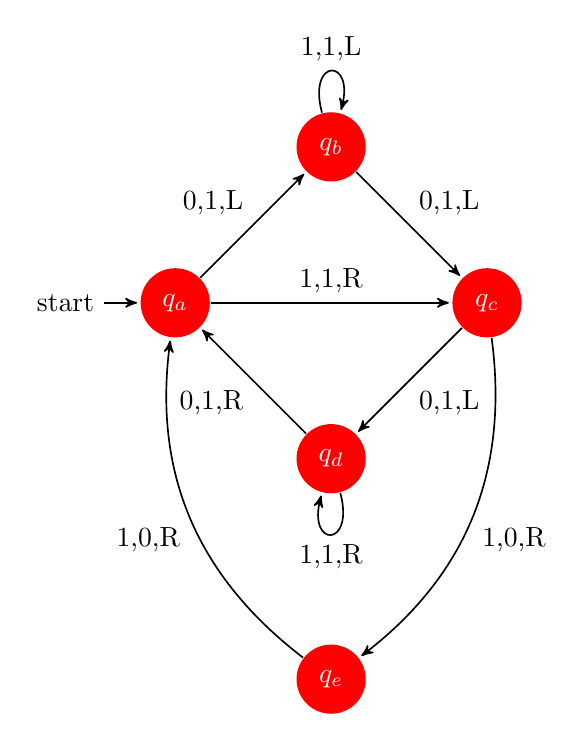
\begin{tikzpicture}[->,>=stealth',shorten >=1pt,auto,node distance=2.8cm,
                    semithick]
  \tikzstyle{every state}=[fill=red,draw=none,text=white]

  \node[initial,state] (A)                    {$q_a$};
  \node[state]         (B) [above right of=A] {$q_b$};
  \node[state]         (D) [below right of=A] {$q_d$};
  \node[state]         (C) [below right of=B] {$q_c$};
  \node[state]         (E) [below of=D]       {$q_e$};

  \path (A) edge              node {0,1,L} (B)
            edge              node {1,1,R} (C)
        (B) edge [loop above] node {1,1,L} (B)
            edge              node {0,1,L} (C)
        (C) edge              node {0,1,L} (D)
            edge [bend left]  node {1,0,R} (E)
        (D) edge [loop below] node {1,1,R} (D)
            edge              node {0,1,R} (A)
        (E) edge [bend left]  node {1,0,R} (A);
\end{tikzpicture}
\end{center}
Koristeći \texttt{sagetex} i okruženje \texttt{automata} možemo definirati jedan automat na sljedeći način: 
\begin{sageblock}
A = Automaton([('P', 'Q', 0), ('P', 'P', 1),
                ('Q', 'P', 1), ('Q', 'Q', 0)],
               initial_states=['P'], final_states=['Q'])
\end{sageblock}
Početno stanje je stanje $P$, a konačno stanje je označeno s $Q$. 
Ako DKA definiramo sa: 
\begin{sageblock}
M = Automaton({'A': [('A', 0), ('B', 1), ('B', -1)], 'B': [('A', 0)]})
\end{sageblock}
tada je zapravo zadana funkcija prijelaza $\delta$, te s:
\begin{sageblock}
M.state('A').is_initial = True
\end{sageblock}
provjeravamo je li $A$ početno stanje, dok s:
\begin{sageblock}
M([1, -1])
sage: False
M([0, -1, 0, 1])
sage: True
\end{sageblock}
vidimo da automat M prihvaća prvi ulaz, odnosno odbija drugi  ulaz.

\section{Istovjetnost stanja}
\textbf{Definicija 2.1.} Neka je $M$ neki DKA zadan s $M = (Q, \Sigma, \delta, q_0, F)$, te $p$ stanje iz $Q$. Kažemo da je stanje $p$\textit{istovjetno} stanju $p'$ DKA $M'= (Q', \Sigma, \delta', q_0', F')$ ako i samo ako DKA $M$ u stanju $p$ prihvaća isti skup nizova kao i DKA $M'$ u stanju $p'$. Za bilo koju riječ $w$ skupa $\Sigma^*$ vrijedi:
\begin{align}\label{eq1}
\delta(p,w) \in F & \wedge \delta'(p',w) \in F'
\end{align}
\begin{align*}ili 
\end{align*}
\begin{align}\label{eq2}
\delta(p,w) \notin F & \wedge \delta'(p',w) \notin F  
\end{align}
\textbf{Napomena. }Relacija istovjetnosti je tranzitivna relacija, tj. ako je stanje $p$ istovjetno stanju $q$ i stanje $q$ istovjetno stanju $r$, tada je stanje $p$ istovjetno stanju $r$. Svojstvo tranzitivnosti nam je važno zbog postupka redukcije broja stanja DKA. 
\newline
\newline
Postupak redukcije može se opisati u tri koraka: 
\begin{enumerate}
\item Sva istovjetna stanja označimo zajedničkim imenom izabranim u prethodnom koraku
\item Sve oznake istovjetnih stanja u funkciji prijelaza $\delta$ označe se izabranim zajedničkim imenom
\item U skupu $Q$ ostavi se samo jedno od istovjetnih stanja, a sva ostala istovjetna stanja se izuzmu. 
\end{enumerate}
Na slici 3 možemo vidjeti postupak redukcije za istovjetna stanja $p_4$ i $p_5$. 
\begin{figure}[h]
\centering
\includegraphics[width=0.8\textwidth, height= 4.5cm]{Postupak.jpg}
\caption{Pojednsotavljenje DKA odbacivanjem jednog od istovjetnih stanja. 
}
\end{figure}
\newline
\newline Prirodno nam se nameće pitanje: "Možemo li proširiti definiciju istovjetnosti stanja na istovjetnost DKA?" Odgovor je pozitivan i dan sljedećim teoremom.  
\newline
\begin{thm} Dva DKA $M$ i $M'$ su \textit{istovjetna} ako i samo ako njihova početna stanja istovjetna. 
\end{thm}
Ispitivanje istovjetnosti stanja $p$ i $q$ svodi se na ispitivanje dva uvjeta: 
\begin{enumerate}
\item \textit{Uvjet podudarnosti:} Stanja $p$ i $q$ moraju biti oba prihvatljiva ($p \in F \wedge q \in F$) ili neprihvatljia  ($p \notin F \wedge q \notin F$)
\item \textit{Uvjet napredovanja:} Za bilo koji ulazni znak $a$ vrijedi da su stanja $\delta(p,a)$ i $\delta(q,a)$ istovjetna.
\end{enumerate}
\begin{corollary}DKA je minimalan ako i samo ako vrijedi da je L(q) različito od L(q') za bilo koja dva različita stanja p i p'. \end{corollary}
\begin{proof}
$\Rightarrow$ Neka je A minimalan DKA. Svaki rezidual od L(A) je prepoznaje barem jedno od stanje od A. Kako je A minimalan, tada on ima brojna stanja, označimo ih s $C_L$, te vrijedi da je broj stanja jednak broju reziduala od L(A). Slijedi, broj različitih stanja od A prepoznaje različite reziduale od L(A).


$\Leftarrow$ Neka je A DKA takav da za različita stanja prepoznaje različite jezike. S obzirom da je svako stanje od A prepoznaje rezidual od L(A), i svaki rezidual od L(A) je prepoznatljiv nekim stanjem od A, broj stanja od jednak je broju reziduala od L(A). Slijedi, A ima jednako stanja kao i $C_L$, pa je minimalan.

\end{proof}
\section{Određivanje istovjetnih stanja}
Sada ćemo obraditi osnovni algoritam za određivanje istovjetnih stanja. Te njegovu implementaciju u Pythonu. 
\newline
\textbf{Algoritam:} Algoritam se zasniva na ispitivanju prethodno navedenih uvjeta podudarnosti i napredovanja koji slijede iz ~\eqref{eq1} i~\eqref{eq2}. Uvjeti se ispituju za sve parove stanja DKA. 
\begin{figure}[h]
\centering
\includegraphics[width=0.6\textwidth]{uvjeti_1.png}
\caption{Implementacija uvjeta podudarnosti u Pythonu}
\end{figure}
\begin{figure}[h]
\centering
\includegraphics[width=0.5\textwidth]{uvjeti_2.png}
\caption{Implementacija uvjeta napredovanja u Pythonu za stanja $p$ i $q$ istog DKA}
\end{figure}
\newline
S obzirom da  je potrebno ispitati sve parove stanja ovaj agoritam se smatra neučinkovitim te postoje poboljšanja. Tim algoritmima se nećemo baviti već se mogu pronaći u \cite{c1}.
\newline
Prepostavimo da ispitujemo jesu li stanja $p_0$ i $p_7$ DKA datog na slici 3 istovjetna. 
Algoritam se izvodi u sljedećim koracima: 
\begin{enumerate}
\item Tablica namijenjena ispitivanju istovjetnosti parova stanja gradi se tako da se za svaki ulazni znak igradi zasebni stupac. Izaberu se dva stanja za koja se želi ispitati istovjetnost, te se taj par upiše u prvi redak. 
\begin{figure}[h]
\centering
\includegraphics[]{1korak.png}
\caption{Stvaranje novog retka u tablici implementirano je u Pythonu sa funkcijom \texttt{iduci\_korak}. Funkcija za par stanja izvodi akciju upravo u ovisnosti o tablici ispod slike.}
\end{figure}
\item Uvjet podudarnosti ispituje se za sve parove novih stanja koji su zapisani u tablicu u prethodnom koraku. Ako par stanja nije podudaran, onda se odrede stanja za sve ulazne znakove, te se ti parovi upišu u odgovarajuće stupce tablice. Na primjer, za par stanja ($p$,$q$) i ulazni znak $a$, u stupac ulaznog znaka $a$ upiše se novi par stanja $(\delta(p,a), \delta(q,a))$.

\item Ako su nova stanja u zadovoljila uvjet podudarnosti, novi par stanja u drugom koraku imamo tri mogućnosti dane u donjoj tablici.  
\newline
\begin{tabular}{p{8cm} | p{8cm}}
\textbf{Par stanja} & \textbf{Akcija} \\
Ista stanja & Nema akcije \\
Različita stanja za koje postoji zapis u jednom od prethodnih redaka & Nema akcije \\
Različita stanja za koje ne postoji zapis u jednom od prethodnih redaka & Stvori novi redak u tablici i upiši u njega novi par stanja
\end{tabular}
\begin{figure}[h]
\centering
\includegraphics[width=0.2\textwidth, height= 1.2cm]{prviprolaz.jpg}

\caption{Na slici možemo vidjeti primjer popunjavanja prvog retka u tablici kada vrijedi
$\delta(p_0, c)$ = $p_0$, $\delta(p_7, c) = p_6, \delta(p_0, d)\ =\ p_3, \delta(p_0, c)\ =\ p_0$}
\end{figure}
\item Ako se u trećem koraku ne zapiše niti jedan novi redak u tablici, onda je par stanja zapisan u prvom retku tablice istovjetan, kao i svi parovi stanja zapisani u ostalim recima tablice. Ostali parovi stanja su istovjetni jer vrijedi uvjet napredovanja. 
\newline
Ukoliko je novi redak zapisan u tablicu, algoritam nastavlja s drugim korakom. 
\begin{figure}[h]
\centering
\includegraphics[height = 7cm]{2korak.png}
\caption{Funkcija \texttt{istovjetna} za nova dva stanja u tablici isputuje njihovu istovjetnost koristeći uvjet podudarnosti.}
\end{figure}
\end{enumerate}
\newpage
Na našem primjeru ispitivanja stanja $p_0$ i $p_7$ u drugom koraku drugog prolaza imamo ispitivanje podudarnost stanja $p_0$ i $p_6$. Budući da stanja $p_0$ i $p_6$ nisu podudarna, stanja $p_0$ i $p_7$ nisu istovjetna i algoritam se zaustavlja. U ovom slučaju funkcija \texttt{istovjetna} bi za stanja $p_0$ i $p_7$ vratila vrijednost \texttt{False} .
\newline \textit{2.prolaz }
\begin{figure}[h]
\centering
\includegraphics[width=0.2\textwidth, height= 1.5cm]{prviprolaz.jpg}
\caption{($p_0 \notin F \wedge p_6 \in F) \Rightarrow stanja$
\newline $p_0$ i $p_7$ nisu istovjetna $ \Rightarrow $ ALGORITAM SE ZAUSTAVLJA}
\end{figure}
\newline
Na slici je dokazana istovjetnost sljedećih parova stanja: ($p_0,p_1$),  ($p_0,p_2$),  ($p_3,p_5$),  ($p_3,p_7$) i  ($p_5,p_7$). Budući da za istovjetnost vrijedi tranzitivnost, na temelju istovjetnosti para stanja ($p_0, p_1$) i para stanja ($p_0, p_2$), par stanja ($p_1, p_2$) također je istovjetan. DKA prikazan na slici 2.10. pojednostavni se na sljedeći način: stanja $p_0,\ p_1 i\ p_2$ zamijene se stanjem A, a stanja $p_3,\ p_5\ i\ p_7$ zamijene se stanjem B. Pojednostavljani DKA prikazan je na slici 11 desno.
\begin{figure}[h]
\centering
\includegraphics[width=0.6\textwidth]{2_9.jpg}
\caption{Prethodno opisan DKA čija su istovjetna stanja $p_0$, $p_1$, $p_2$ zamijenjena slovom A, a $p_3$, $p_5$, $p_7$ slovom B.}
\end{figure}

\begin{figure}[h]
\centering
\includegraphics[width=0.6\textwidth]{2_10.jpg}
\caption{Postupak dokazivanja istovjetnosti stanja $p_0$ i $p_1$ DKA datog na slici 10.}
\end{figure}
Implementacija minimizacije DKA dana je funkcijom \texttt{minimiziraj}. Zamijena istovjetih stanja radi uz pomoć fukcije \texttt{podijeli} koja jednostavno sva istovjetna stanja grupira u isti skup. Funkcija \texttt{minimiziraj} koristi tu informaciju kao rječnik te sva istovjetna stanja zamijeni s predstavnikom skupa (tj. s prvim stanjem skupa istovjetnih stanja).  
\begin{figure}[h]
\centering
\includegraphics[width=0.8\textwidth]{minimiziraj.png}
\caption{Postupak dokazivanja istovjetnosti stanja $p_0$ i $p_1$ DKA datog na slici 10.}
\end{figure}
\begin{figure}[h]
\centering
\includegraphics[width=\textwidth, height = 1.5cm]{izrezak.png}
\caption{Za primjer iz \cite{c1}, strana 28, slika 2.8. pokretanjem našeg programa dobijemo minimizirani DKA.}
\end{figure}
\newpage
\section{Nedohvatljiva stanja}
\textbf{Definicija 4.1.} Za stanje $p$ DKA $M = (Q, \Sigma, \delta, q_0, F)$ kažemo da je \textit{nedohvatljivo} ako ne postoji niti jedan niz $w \in \Sigma^*$ za koji vrijedi da je $p = \delta(q_0,w)$. Stanje $p_4$ DKA sa slike 2.10 je primjer nedohvatljivog stanja. Odbacivanjem nedohvatljivih stanja dobije se istovjetni DKA  manjim brojem stanja. Dohvatljiva stanja DKA $M = (Q, \Sigma, \delta, q_0, F)$ određuju se sljedećim algoritmom: 
\begin{enumerate}
\item U listu dohvatljivih stanja DS upiše se početno stanje $q_0$.
\item Lista stanja DS proširi se skupom stanja \{ p | p = $\delta(q_0, a),\ za\ sve a \in \Sigma$\}
\item Za sva stanja $q_i \in DS$ proširi se lista skupom stanja $\{ p | p = \delta(q_0, a),$ stanje p nije prethodno zapisano u listu, za sve $a \in \Sigma\}$
\end{enumerate}
Ako se lista dohvatljivih stanja DS proširi zapisom novog stanja, onda se rad algoritma nastavlja korakom (3). Lista DS sadrži sva dohvatljiva stanja, dok su ostala stanja nedohvatljiva. 
\newline
\textit{Primjer rada algoritma.}
\begin{enumerate}
\item korak DS: \textbf{$q_0  $}
\item korak DS: \textbf{$q_0$, $q_1$, $q_5  $} 
\newline jer je $\delta(q_0,c) = q_1$, $\delta(q_0,d) = q_5$
\item korak DS: \textbf{$q_0$, $q_1$, $q_5$, $q_2$, $q_7$, $q_3$} 
\newline jer je $\delta(q_1,c) = q_2$, $\delta(q_1,d) = q_7$ i $\delta(q_5,c) = q_3$
\item korak DS: \textbf{$q_0$, $q_1$, $q_5$, $q_2$, $q_7$, $q_3 $} 
\newline DS se ne mijenja, jer stanja $q_2$, $q_7$ i $q_3$ ne prelaze u niti jedno stanje koje od prije nije zapisano u listu, i rad algoritma se nastavlja. 
\end{enumerate}
Nedohvatljiva stanja $q_4$, $q_6$ i $q_8$ se odbacuju.  
\newpage
\section{DKA s minimalnim brojem stanja}
Odbacivanjem istovjetnih i nedohvatljivih stanja dobije se istovjetni DKA s minimalnim brojem stanja. Ne postoji niti jedan drugi DKA koji prihvaća drugi jezik, a ima manji broj stanja. Budući da je postupak odbacivanja nedohvatljivih stanja jednostavniji od postupka odbacivanja istovjetnih stanja, te budući da se odbacivanjem nedohvatljivih stanja smanjuje ukupni broj stanja, što pojednostavljuje postupak odbacivanja istovjetnih stanja, učinkovitije je najprije primijeniti postupak opdvacivanja nedohvatljivih stanja, a zatim postupak odbacivanja istovjetnih stanja. 




Za kraj prikažimo još jednom proširenje DKA tako da mu dodamo još novo istovjetno stanje. 
\begin{center}
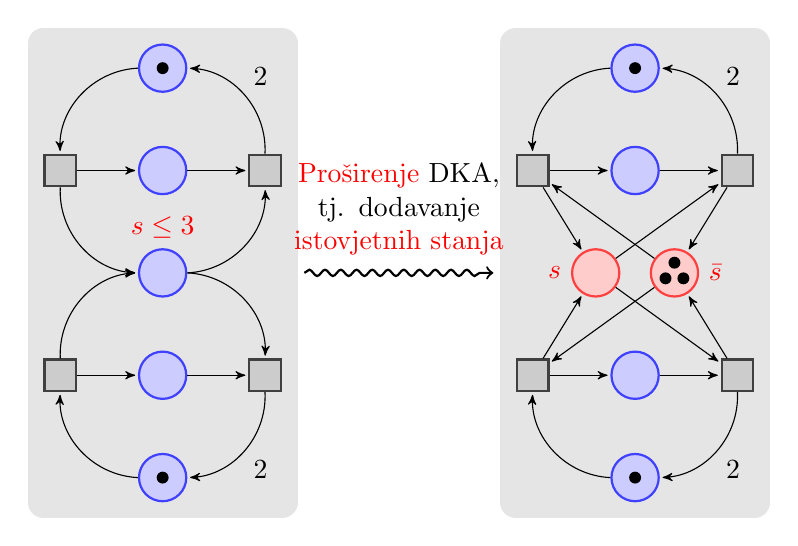
\begin{tikzpicture}[node distance=1.3cm,>=stealth',bend angle=45,auto]

  \tikzstyle{place}=[circle,thick,draw=blue!75,fill=blue!20,minimum size=6mm]
  \tikzstyle{red place}=[place,draw=red!75,fill=red!20]
  \tikzstyle{transition}=[rectangle,thick,draw=black!75,
  			  fill=black!20,minimum size=4mm]

  \tikzstyle{every label}=[red]

  \begin{scope}
    % First net
    \node [place,tokens=1] (w1)                                    {};
    \node [place] (c1) [below of=w1]                      {};
    \node [place] (s)  [below of=c1,label=above:$s\le 3$] {};
    \node [place] (c2) [below of=s]                       {};
    \node [place,tokens=1] (w2) [below of=c2]                      {};

    \node [transition] (e1) [left of=c1] {}
      edge [pre,bend left]                  (w1)
      edge [post,bend right]                (s)
      edge [post]                           (c1);

    \node [transition] (e2) [left of=c2] {}
      edge [pre,bend right]                 (w2)
      edge [post,bend left]                 (s)
      edge [post]                           (c2);

    \node [transition] (l1) [right of=c1] {}
      edge [pre]                            (c1)
      edge [pre,bend left]                  (s)
      edge [post,bend right] node[swap] {2} (w1);

    \node [transition] (l2) [right of=c2] {}
      edge [pre]                            (c2)
      edge [pre,bend right]                 (s)
      edge [post,bend left]  node {2}       (w2);
  \end{scope}

  \begin{scope}[xshift=6cm]
    % Second net
    \node [place,tokens=1]
                      (w1')                                                {};
    \node [place]     (c1') [below of=w1']                                 {};
    \node [red place] (s1') [below of=c1',xshift=-5mm,label=left:$s$]      {};
    \node [red place,tokens=3]
                      (s2') [below of=c1',xshift=5mm,label=right:$\bar s$] {};
    \node [place]     (c2') [below of=s1',xshift=5mm]                      {};
    \node [place,tokens=1]
                      (w2') [below of=c2']                                 {};

    \node [transition] (e1') [left of=c1'] {}
      edge [pre,bend left]                  (w1')
      edge [post]                           (s1')
      edge [pre]                            (s2')
      edge [post]                           (c1');

    \node [transition] (e2') [left of=c2'] {}
      edge [pre,bend right]                 (w2')
      edge [post]                           (s1')
      edge [pre]                            (s2')
      edge [post]                           (c2');

    \node [transition] (l1') [right of=c1'] {}
      edge [pre]                            (c1')
      edge [pre]                            (s1')
      edge [post]                           (s2')
      edge [post,bend right] node[swap] {2} (w1');

    \node [transition] (l2') [right of=c2'] {}
      edge [pre]                            (c2')
      edge [pre]                            (s1')
      edge [post]                           (s2')
      edge [post,bend left]  node {2}       (w2');
  \end{scope}

  \draw [-to,thick,snake=snake,segment amplitude=.4mm,
         segment length=2mm,line after snake=1mm]
    ([xshift=5mm]s -| l1) -- ([xshift=-5mm]s1' -| e1')
    node [above=1mm,midway,text width=3cm,text centered]
      {\textcolor{red}{Proširenje} DKA, tj. dodavanje
        \textcolor{red}{istovjetnih stanja}};

  \begin{pgfonlayer}{background}
    \filldraw [line width=4mm,join=round,black!10]
      (w1.north  -| l1.east)  rectangle (w2.south  -| e1.west)
      (w1'.north -| l1'.east) rectangle (w2'.south -| e1'.west);
  \end{pgfonlayer}
\end{tikzpicture}
\end{center}



\begin{thebibliography}{99}

\bibitem{c1} Siniša Srbljić, Jezični procesori 1, 2. izdanje,  Zagreb, 2002.
\bibitem{c2} Sipser, Introduction to the theory of computation 2nd edition, Thomson, 2006.
\bibitem{c3} web.math.pmf.unizg.hr/nastava/ip/
\newline Materijali s predavanja kolegija Interpretacija programa

\end{thebibliography}

\end{document}